% Familytreemap User Guide
%
% For PDF output: pdflatex familytreemap.tex
% For HTML output: plastex familytreemap.tex
%
% For Graphics:
% Use PNG format to avoid problems with HTML conversion.
% Recommended size: < 13cm x 18cm (width x height).
% Recommended resolution: 300 dpi.
%
% Use fixed width instead of textwidth, so that plastex can
% recognize the graphics size. For example use
% \includegraphics[width=13cm]{img/haplogroups.png}
% instead of
% \includegraphics[width=\textwidth]{img/haplogroups.png}

\documentclass[12pt,a4paper]{article}
\usepackage[utf8]{inputenc}
\usepackage[english]{babel}
\usepackage[colorlinks=true, urlcolor=blue, linkcolor=blue]{hyperref}
\usepackage{graphicx}

\begin{document}
\title{Familytreemap User Guide}
\author{Dirk Struve\\
phylofriend at projectory.de\\
\href{https://github.com/yogischogi/familytreemap/}{https://github.com/yogischogi/familytreemap/}}
\date{\today}
\maketitle
\tableofcontents


\section{Introduction}

\hfill {\sl For the lost ones.}
\vspace{1em}

\noindent
Familytreemap calculates population frequencies
(relative or absolute) from Family Tree DNA projects.

It's main purpose is to create heat maps of project members.


\section{Command Line Options}

Familytreemap is a command line program. It is invoked by

\vspace{1em}
\noindent\texttt{familytreemap <options>}

\vspace{1em}
\noindent Options may be given in arbitrary order.

\begin{description}
\item[-help] Prints available program options.
\item[-tin] Input file (testers is) contains the total
  number of testers for each country.
\item[-in] Input file contains a table with Family Tree DNA
  project data in CSV format.
\item[-col] Number of the column that contains the country names.
\item[-out] Output file contains population frequencies in
  CSV format.
\item[-relative] If \texttt{-relative=false} the absolute
  number of testers belonging to a group is calculated.
  Default value is \texttt{-relative=true}.
\item[-sumuk] (sumUK) If \texttt{-sumuk=true} the number of
  testers from England, Wales, Scotland and Northern Ireland
  is added to United Kingdom. Default is \texttt{-sumuk=false}
  because this is the way the data is reported by Family Tree DNA.
\end{description}


\section{Installation}

\subsection{Linux Mint}
\begin{enumerate}
\item Make sure that the Go programming language is installed.
	You can install it by typing\\
	\texttt{sudo apt-get install golang}
\item Read the Go
	\href{http://golang.org/doc/install}{Getting Started}
	guide. Make sure to set your \emph{GOPATH} variable and
	include it in your \emph{PATH} so that Go programs can be
	found.
\item Fetch the familytreemap program with\\
	\texttt{go get github.com/yogischogi/familytreemap}
\item Install the program with\\
	 \texttt{go install github.com/yogischogi/familytreemap}
\end{enumerate}

\subsection{Windows, FreeBSD, Mac OS X}
\begin{enumerate}
\item Read the Go
	\href{http://golang.org/doc/install}{Getting Started}
	guide and install the Go programming language. 
	Make sure to set your \emph{GOPATH} variable and
	include it in your \emph{PATH} so that Go programs can be
	found.
\item Fetch the familytreemap program with\\
	\texttt{go get github.com/yogischogi/familytreemap}
\item Install the program with\\
	 \texttt{go install github.com/yogischogi/familytreemap}
\end{enumerate}


\section{First Usage}

\begin{enumerate}
\item Go to a Family Tree DNA project on the web and open the
  page containing the DNA results in a web browser.
\item Copy the results into a spreadsheet and save it in
  CSV (Comma Separated Values) format. For this example
  name it \emph{projectdata.csv}.
\item Open a command line interpreter and go to the
   directory where your files are.
\item Determine the number of the column which contains
  the countries. Often this is 3, familytreemap's default
  value.
\item Issue a command to test if the program works:\\
  \texttt{familytreemap -in projectdata.csv -out result.csv -col 3}\\
  The program should be working and prompt you to use
  the \texttt{-tin} option to provide the number of total testers
  for each country. Without the \texttt{-tin} option it
  is not possible to calculate an accurate relative distribution.
  Instead the program uses build in example data.
\end{enumerate}


\section{The -tin Option}

To calculate a relative distribution of project members it
is necessary to provide a number for each country which
denotes the total number of testers from that country.

This is done by using the \texttt{-tin} option and providing
a file in JSON format that contains country names and the
total number of testers. A very simple example file for just
three countries looks like this:

\begin{verbatim}
{"Belarus":1000,
"Belgium":2000,
"Brazil":100}
\end{verbatim}

\noindent
A good way to get the number of testers for each country 
is to sign into Family Tree DNA and go to \emph{Ancestral Origins}.
If you have completed your \texttt{-tin} file, you can
name it for example \emph{totals.json} and provide it to
the program like this:

\vspace{1ex}
\noindent
\texttt{familytreemap -tin totals.json -in projectdata.csv -out result.csv -col 3}
\vspace{1ex}

\noindent
The program should be fully working now.


\section{How to Create a Heat Map}

\begin{figure}[ht]
\centering
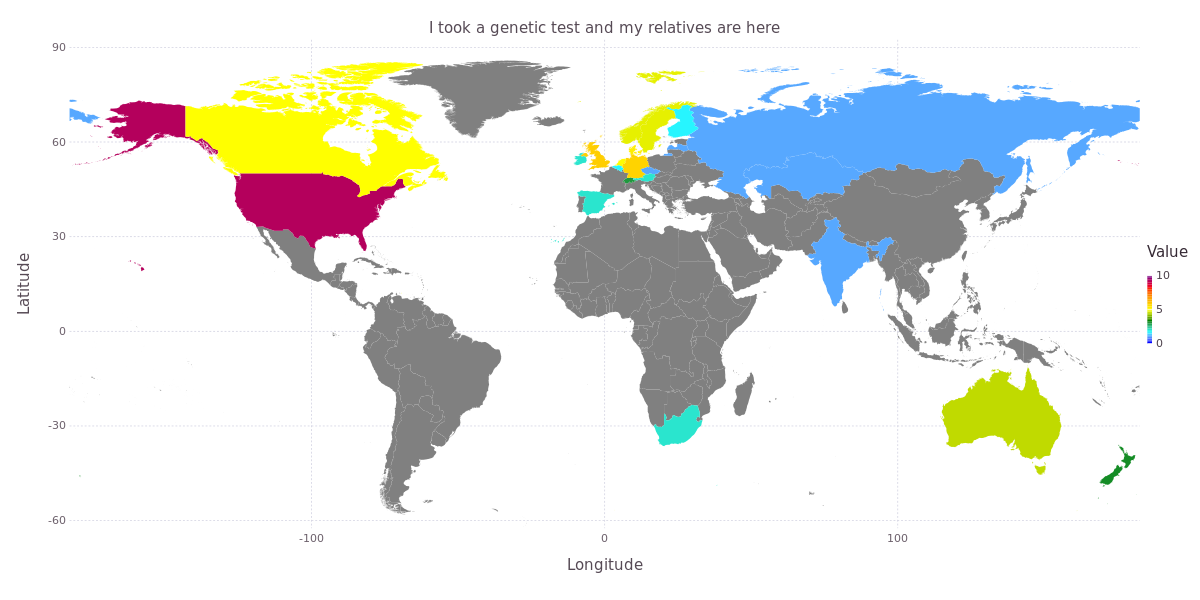
\includegraphics[width=13cm]{heatmap.png}
\caption{Geographical distribution of persons belonging
to a haplogroup. Created with \href{http://www.openheatmap.com/}{OpenHeatMap}.}
\end{figure}

\begin{enumerate}
\item Run the familytreemap program:\\
  \texttt{familytreemap -tin totals.json -in projectdata.csv -out result.csv -col 3}
\item Open your web browser and go to
      \href{http://www.openheatmap.com/}{http://www.openheatmap.com}.
	\begin{enumerate}
	\item Click on \emph{Create your map}.
	\item \emph{Excel or CSV file}.
	\item \emph{Upload} your results file,
            in this example \emph{result.csv}.
	\item \emph{View your map} and adjust the settings until you like it.
	\item \emph{Save \& view}
	\end{enumerate}
\item You are done! You can share your map via social networks
  or take a screenshot of it.
\end{enumerate}


\end{document}
